\documentclass[dvipdfmx,12pt]{beamer}
\usepackage{lipsum}
\usetheme{Verona}
\usepackage{bxdpx-beamer}
\usepackage{pxjahyper}
\usepackage{minijs}
\usepackage{mathpazo}
\usepackage{amsmath,amssymb}
\usepackage{graphicx}
\graphicspath{{fig_tab/os20221215/}}
\usepackage{array}
\usepackage{tikz}
\usepackage{wrapfig}
\usepackage{float}
\usepackage{here}
\usepackage{lscape}
\usepackage{ascmac}
\usepackage{siunitx}
\usepackage{tabularx}
\renewcommand{\kanjifamilydefault}{\gtdefault}
\hypersetup{% hyperrefオプションリスト
 setpagesize=false,
 bookmarksnumbered=true,%
 bookmarksopen=true,%
 colorlinks=true,%
 linkcolor=blue,
 citecolor=blue,
 urlcolor = magenta
}
\setbeamertemplate{navigation symbols}{}

\title[Currie, Voorheis, and Walker, Forthcoming]{What Caused Racial Disparities \\ in Particulate Exposure to Fall?}
\subtitle{New Evidence from the Clean Air Act \\ and Satellite-Based Measures of Air Quality}
\author[R.Tanji]{Currie, Voorheis, and Walker (AER, Forthcoming): Reviewed by R. TANJI}
\date[12/15/2022 OS Semi.]{December 15th, 2022 \\ Ohtake-Sasaki Seminar}
\institute[]{Osaka University, Graduate School of Economics}

\begin{document}

\begin{frame}\frametitle{}
\titlepage
\end{frame}

\section{Introduction}

\begin{frame}\frametitle{Abstract}
  \begin{itemize}
    \item This paper examines the underlying structure that causes racial differences in exposure to ambient air pollution in the United States.
    \begin{itemize}
      \item The difference have declined significantly over the past 20 years.
    \end{itemize}
    \item Clean Air Act (CAA) explains the excess convergence in Black-White pollution exposure
    \begin{itemize}
      \item Areas with larger Black populations saw greater CAA-related declines in PM2.5 exposure
      \item Over 60\% of the reduction in the racial convergence in PM2.5 pollution exposure since 2000
    \end{itemize}
  \end{itemize}
\end{frame}

\frame{\tableofcontents}

\frame{\sectionpage}
\begin{frame}{Motivation \& Literature}
  \begin{itemize}
    \item The existing evidence about racial disparities in pollution exposure is largely piecemeal and indirect.
    \begin{itemize}
      \item Low income and/or racial minorities in the U.S. have been exposed to environmental burdens (Office, 1983; Chavis and Lee, 1987)
      \item Lack of monitoring device to track small particulates (Fowlie, Rubin, and Walker, 2019)
      \item Alternative measurement: distance to a polluting facility
    \end{itemize}
    \item Moreover, we know very little about why racial gaps in pollution exposure may have changed over time.
  \end{itemize}
\end{frame}

\begin{frame}{This Paper}
  \begin{itemize}
    \item Data: newly available national data on PM2.5 exposure from 2000 to 2015
    \begin{itemize}
      \item 1km-grid measures of ambient air pollution levels for the entire United States
    \end{itemize}
    \item Analyses
    \begin{enumerate}
      \item Document racial gaps in ambient exposure to PM 2.5 and the time-series changes between 2000 and 2015.
      \item Explain the gaps by differences in individual and/or neighborhood characteristics.
      \item Explore the contribution of changes in \textbf{relative mobility} and \textbf{relative improvements} in neighborhood air quality.
      \item Use quantile regression to see the impact of the Clean Air Act and National Ambient Air Quality Standards (NAAQS).
    \end{enumerate}
  \end{itemize}
\end{frame}

\begin{frame}{Summary of Results}
  \begin{enumerate}
    \item African Americans tend to live in the most polluted areas nationally, but the gap has been closing.
    \begin{itemize}
      \item Mean gap in pollution exposure: \SI[per-mode=symbol]{1.5}{\micro \gram \per \cubic \meter} $\rightarrow$ \SI[per-mode=symbol]{0.5}{\micro \gram \per \cubic \meter}
    \end{itemize}
    \item differences in individual or household-level characteristics such as income, explain only a tiny part of observed convergence in pollution levels.
    \begin{itemize}
      \item relative mobility differences or changes in Black-White population shares are not able to explain the observed convergence in pollution exposure
    \end{itemize}
    \item Much of this improvement of air quality around African Americans' is driven by the introduction of the PM2.5 NAAQS.
    \begin{itemize}
      \item Spatially targeted nature of the CAA regulations contributes to the observed convergence in
      mean PM2.5 differences between Blacks and Whites.
    \end{itemize}
  \end{enumerate}
\end{frame}

\begin{frame}{Contributions}
  \begin{enumerate}
    \item The first paper to link national representative survey to nationwide grid of PM 2.5 mesurement.
    \begin{itemize}
      \item Explored the causal determinants of narrowing pollution gaps between racial groups over time.
      \item Explore how much variation in pollution exposure be explained by individual endowments (income), aggregate neighborhood-level (average years of schooling) characteristics.
      \item External validity (the spatially continuous PM2.5 measurements)
    \end{itemize}
  \end{enumerate}
\end{frame}

\begin{frame}{}
  \begin{enumerate}
    \setcounter{enumi}{1}
    \item Effects of environmental policy
    and the Clean Air Act more specifically
    \begin{itemize}
      \item Previous literature estimates average effects of policies (Chay and Greenstone, 2003; Isen, Rossin-Slater, and Walker, 2017)
      \item Applying unconditional quantile regression(Firpo, Fortin, and Lemieux, 2009), they can discuss the impact of the Clean Air Act on diffrent empirical moments of the nationwide pollution distribution
    \end{itemize}
  \end{enumerate}
\end{frame}

\section{Data}
\frame{\sectionpage}
\begin{frame}{Background and Difficulties}
  \begin{itemize}
    \item Spatially-continuous satellite measurements of pollution correlates
    \begin{itemize}
      \item "out-of-sample" predictions: build a predictive model of a pollutant of interest by correlating EPA-monitor data with the observable characteristics (van Donkelaar, Martin, Brauer et al, 2016)
    \end{itemize}
    \item This paper uses a 1km by 1km resolution daily PM2.5 concentration data of 2000-2015 (Di, Kloog, Koutrakis et al., 2016).
    \begin{itemize}
      \item Satellite measurements are biased downward for high PM2.5 levels.
    \end{itemize}
  \end{itemize}
\end{frame}

\begin{frame}{Data Construction}
  \begin{itemize}
    \item Individual-level data with pollution and racial identities
    \begin{itemize}
      \item 2000 Census long from
      \item 2001-2015 American Community Surveys
    \end{itemize}
    \item Primary comparisons focus on the non-Hispanic White and African American populations.
    \begin{itemize}
      \item These are the largest and most-documented gaps
      \item Lieber, Porter, Fernandez et al., 2017: Hispanic identity is more fluid over time than White or black racial identities.
    \end{itemize}
  \end{itemize}
\end{frame}

\begin{frame}{}
  \begin{figure}
    \centering
    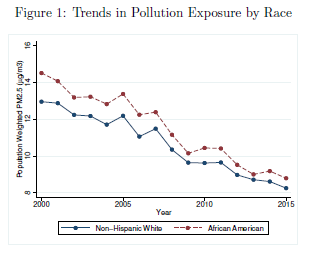
\includegraphics[scale = 1]{F1.png}
    % 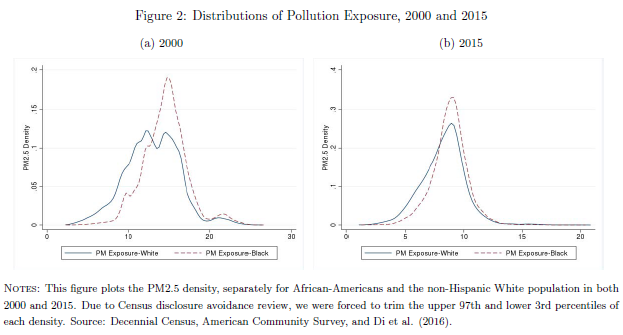
\includegraphics[scale = .5]{F2.png}
  \end{figure}
\end{frame}

\begin{frame}{Racial Gaps in Pollution Exposure}
  \begin{itemize}
    \item The observed racial gap in mean pollution exposure has declined by \SI[per-mode=symbol]{1.0}{\micro \gram \per \cubic \meter}  in 15 years.
    \item This improvement in the Black-White pollution gap could potentially explain 4\% of the mortality gap improvement.
    \begin{itemize}
      \item Life expectancy is reduced by .61 years for each \SI[per-mode=symbol]{10}{\micro \gram \per \cubic \meter} (Pope III, Ezzati, and Dockery, 2015)
      \item Over 2000-2015, the Black-White gap in life expectancy fell from about 5 years to 3.5 years (Arias, Xu, and Kochanek, 2019).
    \end{itemize}
    \item The gap in exposure is explained by census-tract differences (about \SI{5}{\square \kilo \meter}).
  \end{itemize}
\end{frame}

\begin{frame}{}
  \begin{figure}
    \centering
    % 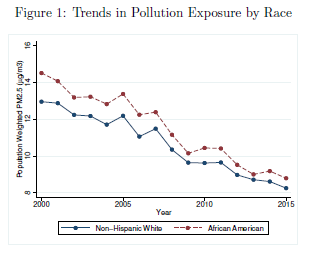
\includegraphics[scale = .1]{F1.png}
    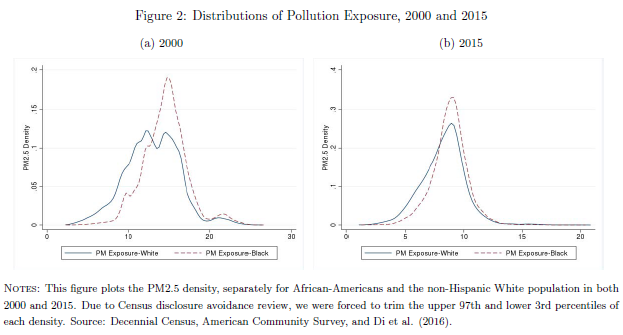
\includegraphics[scale = .7]{F2.png}
  \end{figure}
\end{frame}

\section{Decomposing Differences in Pollution Exposure}
\frame{\sectionpage}
\begin{frame}{}
  \begin{figure}
    \centering
    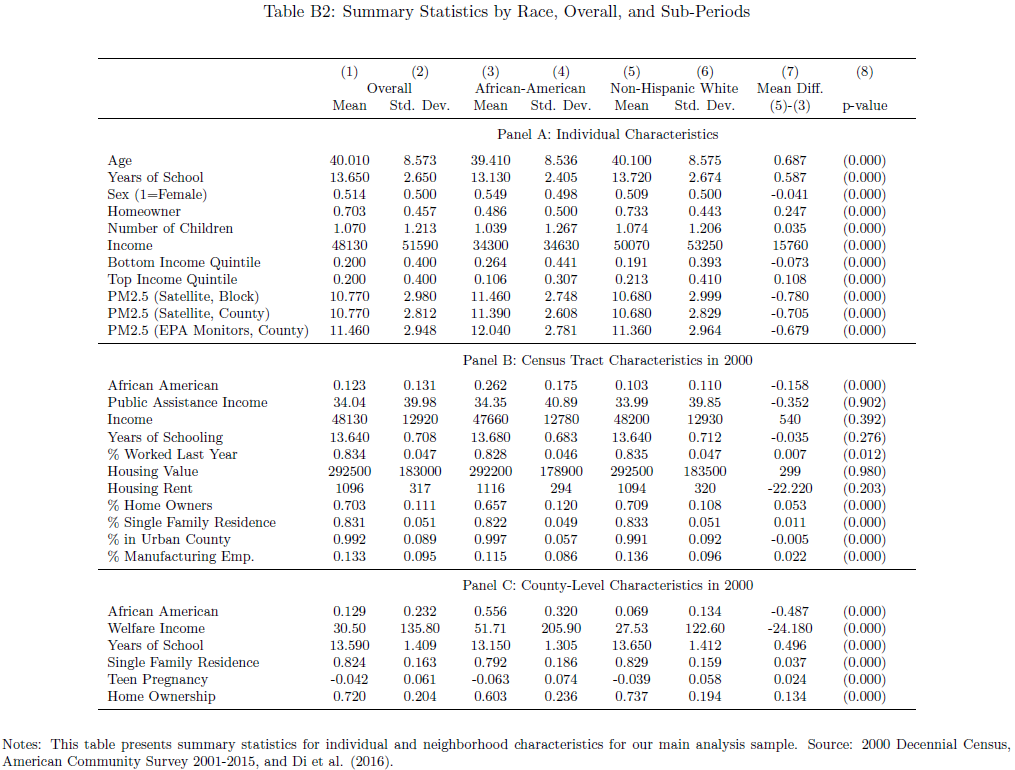
\includegraphics[scale = .4]{TB2.png}
  \end{figure}
\end{frame}

\begin{frame}{Conditional versus Unconditional Differences in Pollution Exposure}
  \begin{itemize}
    \item Differences in exposure conditional on the differences in individual characteristics.
    \item Linear Regression: for individual $i$,
    \begin{align*}
      P_i = \gamma \mathbb{1}[\text{African American}_i] + X' \beta + \epsilon_i
    \end{align*}
    \begin{itemize}
      \item $X_i$: individual income, age, education, number of children, gender, and an indicator for homeownership.
      \item weighted by survey weights
      \item SEs are clustered by commuting zone
    \end{itemize}
  \end{itemize}
\end{frame}

\begin{frame}{}
  \begin{figure}
    \centering
    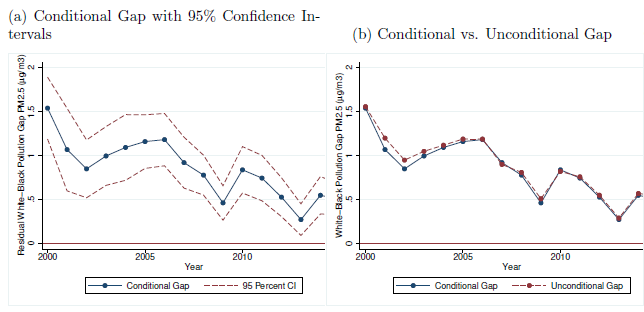
\includegraphics[scale = 1]{F3AB.png}
  \end{figure}
  \begin{itemize}
    \item Individual characteristics seems to explain almost none of the differences.
  \end{itemize}
\end{frame}

\begin{frame}{Oaxaca-Blinder decinoisution}
  \begin{itemize}
    \item Formally decomposing cross-sectional differences (Oaxaca, 1973; Blinder, 1973).
    \begin{align*}
      P_b - P_w = (X_b - X_w)\beta_b + (\beta_b - \beta_w)X_w
    \end{align*}
    \item Observable differences in individual and household characteristics are able to explain at most 8 percent of the gap in mean differences in any given year.
  \end{itemize}
\end{frame}

\begin{frame}{}
  \begin{figure}
    \centering
    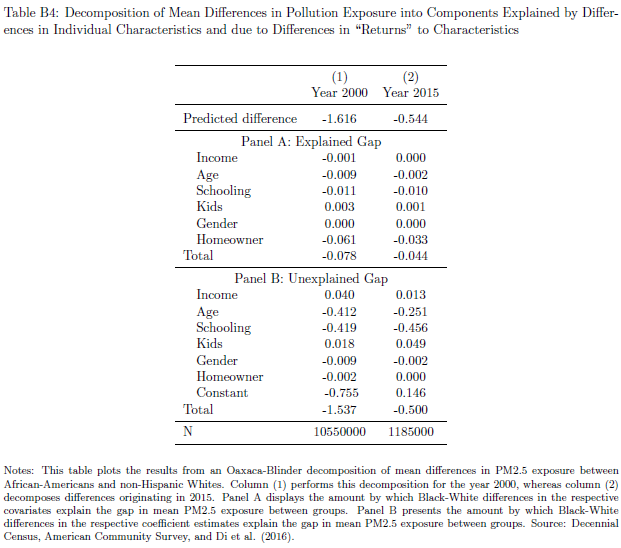
\includegraphics[scale = .6]{TB4.png}
  \end{figure}
\end{frame}

\begin{frame}{Differences at Different Quantiles of the Pollution Distribution}
  \begin{itemize}
    \item Individual or household characteristics are able to explain differences in pollution exposure at other parts of the pollution distribution.
    \item DiNardo, Fortin, and Lemieux (1996): re-weighted kernel density estimate
    \begin{itemize}
      \item estimate what the entire distribution of African American pollution exposure would look like if African Americans had the same observable characteristics
    \end{itemize}
    \item Again, individual characteristics are able to explain little of the observed pollution gap throughout the distribution.
  \end{itemize}
\end{frame}

\begin{frame}{}
  \begin{figure}
    \centering
    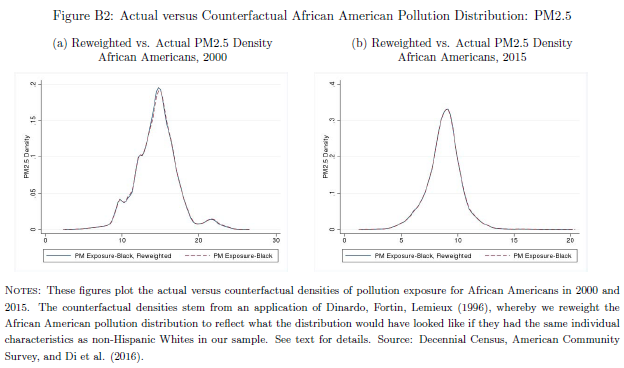
\includegraphics[scale = .6]{FB2.png}
  \end{figure}
\end{frame}

\begin{frame}{Neighborhood Characteristics}
  \begin{itemize}
    \item Socioeconomic Characteristics
    \begin{itemize}
      \item African Americans tend to be concentrated in census tracts with relatively disadvantaged neighbors.
      \item mean public assistance income, the teen pregnancy rate, years of schooling, the share living in single family residences, the home ownership rate, miles of major highways, and total facility PM2.5 emissions
    \end{itemize}
    \begin{figure}
      \centering
      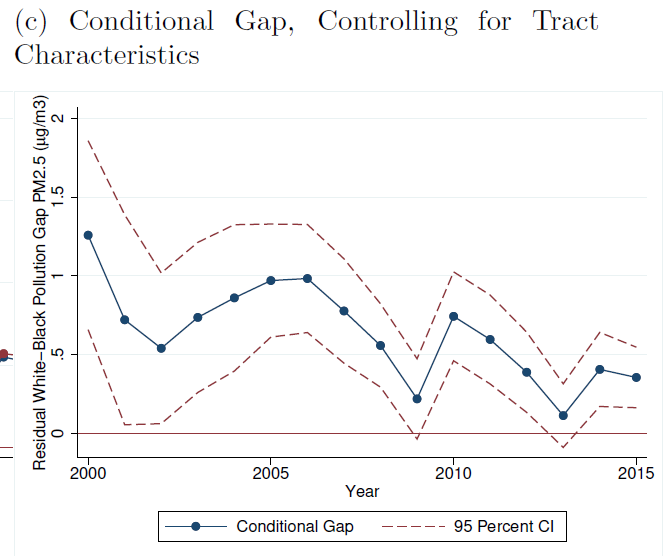
\includegraphics[scale = .4]{F3C.png}
    \end{figure}
  \end{itemize}
\end{frame}

\begin{frame}{}
  \begin{table}
    \begin{tabular}{cc}
      \begin{minipage}{.4\textwidth}
        \begin{itemize}
          \item Black-White differences in neighborhood characteristics explain 0.324 of the documented 1.617 gap in PM2.5 exposure.
          \item tract home ownership rate explain about 20 percent of the difference in PM2.5 exposure.
          \item Education translates into substantially less pollution exposure for Whites than it does for Blacks.
        \end{itemize}
      \end{minipage} &
      \begin{minipage}{.6\textwidth}
        \begin{figure}
          \centering
          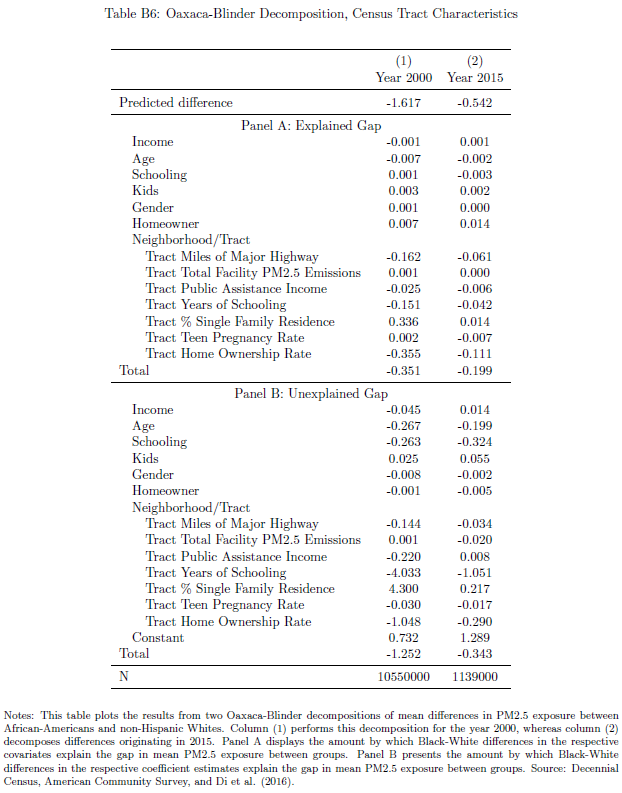
\includegraphics[scale = .4]{TB6.png}
        \end{figure}
      \end{minipage}
    \end{tabular}
  \end{table}
\end{frame}

\begin{frame}{The Role of Relative Mobility}
  \begin{itemize}
    \item Is the improvement due to the relative movement of African Americans?
    \item To compare the counterfactual pollustion exposure in 2015 (without mobility), the authors use Decennial Census.
    \begin{itemize}
      \item Block-level population counts for non-Hispanic Whites and African Americans.
    \end{itemize}
    \item If populations were fixed in their 2000 locations, the gain would have been \SI[per-mode=symbol]{0.89}{\micro \gram \per \cubic \meter} instead of \SI[per-mode=symbol]{1.02}{\micro \gram \per \cubic \meter} (12.7\% of the total improvement.)
    \item The negative relationship between White population shares and pollution levels has weakened over time.
  \end{itemize}
\end{frame}

\begin{frame}{}
  \begin{figure}
    \centering
    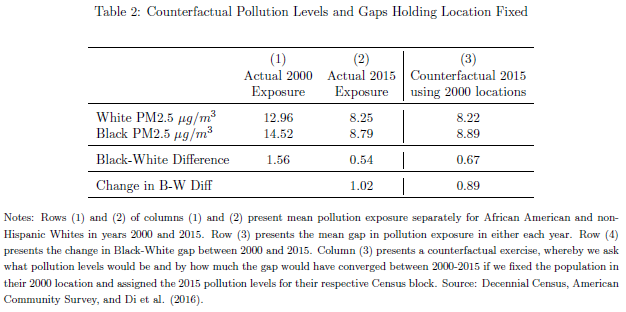
\includegraphics[scale = .7]{T2.png}
  \end{figure}
\end{frame}

\section{The Clean Air Act and Relative Changes in Pollution Exposure}
\frame{\sectionpage}
\begin{frame}{The Clean Air Act and Relative Changes in Pollution Exposure}
  \begin{itemize}
    \item African American neighborhoods appears to have had greater improvements in air quality
    \item Clean Air Act (CAA)
    \begin{itemize}
      \item regulations governing both stationary sources (factories) and mobile sources (cars).
    \end{itemize}
    \item national ambient air quality standards (NAAQS): maximum allowable concentrations of criterion air pollutants (for stationary sources)
    \begin{itemize}
      \item Each in year in July, the set of counties are checked (by EPA) if they violate their standard.
      \item If they violate, the EPA can withhold federal funding for the state.
    \end{itemize}
  \end{itemize}
\end{frame}

\begin{frame}{History of the CAA Policy Changes}
  \begin{itemize}
    \item In 1997, the EPA tightened the NAAQS regulation about PM2.5 for the first time.
    \item After years of controversy in the court, the new standards were implemented in April 2005.
    \begin{itemize}
      \item Revisions of the standard occured in 2006 and went into effect in 2009
    \end{itemize}
    \item Because changes in 2005 was mandatory on reductions in annual PM 2.5, they focus this policy implementation.
  \end{itemize}
\end{frame}

\begin{frame}{Racial Distribution and Pollution Decile}
  \begin{figure}
    \centering
    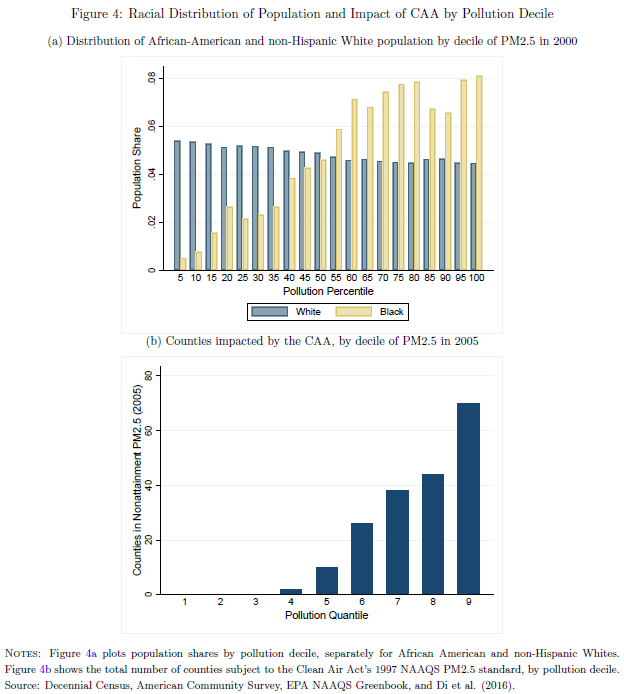
\includegraphics[scale = .4]{F4.png}
  \end{figure}
\end{frame}

\begin{frame}{}
  \begin{figure}
    \centering
    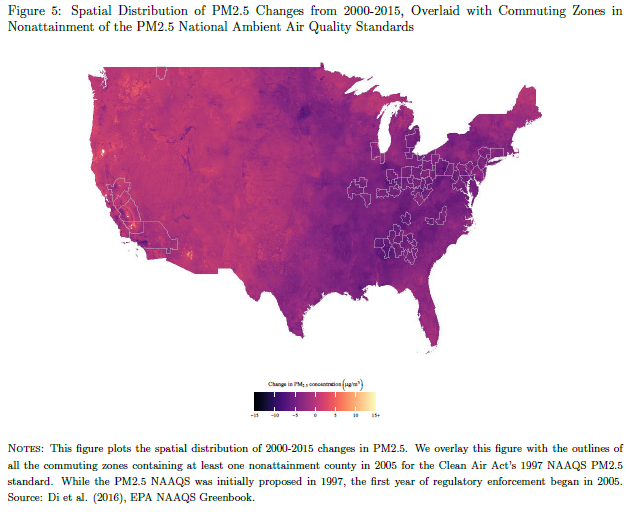
\includegraphics[scale = .6]{F5.png}
  \end{figure}
\end{frame}

\begin{frame}{Impact of CAA: Identification Strategy}
  \begin{itemize}
    \item Standard DID and event-study design
    \item For person $i$ residing commuting zone $c$ in year $t$,
    \begin{align*}
      P_{ict} = \sum_{t = 2000}^{2015} \beta_t (\mathbb{1}[\text{Nonattain}_c] \times \mathbb{1}[\text{year}_t = t]) + \gamma_c + \rho_t + \epsilon_{ict}
    \end{align*}
    \begin{itemize}
      \item 62 CZs consists of 250 counties in 20 states were designated as nonattainment areas.
      \item If the CZ violates the standard of pollutants, the indicator takes one.
      \item weighted by survey weights
      \item SEs are clustered by commuting zone
    \end{itemize}
  \end{itemize}
\end{frame}

\begin{frame}{}
  \begin{figure}
    \centering
    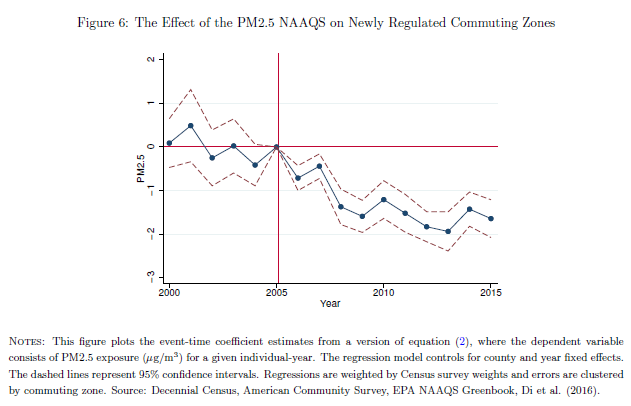
\includegraphics[scale = .6]{F6.png}
  \end{figure}
\end{frame}

\begin{frame}{}
  \begin{figure}
    \centering
    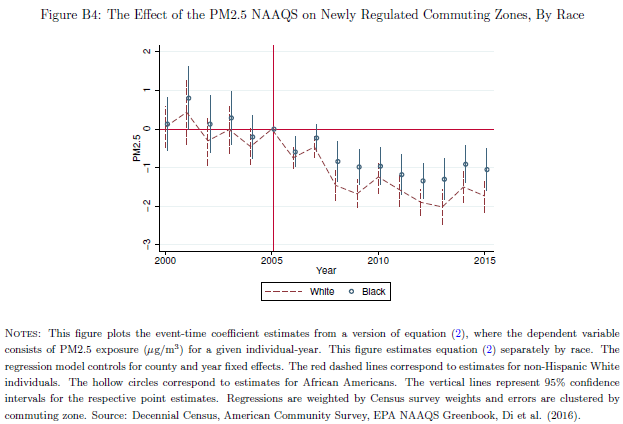
\includegraphics[scale = .5]{FB4.png}
  \end{figure}
  \begin{itemize}
    \item Standard DID
    \begin{align*}
      P_{ict} = \beta (\mathbb{1}[\text{Nonattain}_c] \times \mathbb{1}[\text{year}_t = t]) + \gamma_c + \rho_t + \epsilon_{ict}
    \end{align*}
  \end{itemize}
\end{frame}

\begin{frame}{}
  \begin{figure}
    \centering
    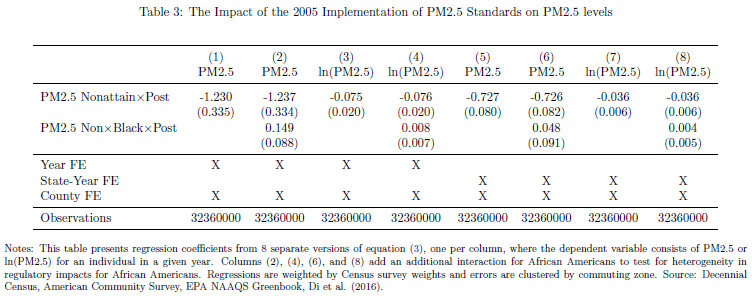
\includegraphics[scale = .6]{T3.png}
  \end{figure}
  \begin{itemize}
    \item Within-county improvements in air quality were slightly less for African Americans than for non-Hispanic Whites (statistically insignificant).
  \end{itemize}
\end{frame}

\begin{frame}{Summary of DID}
  \begin{itemize}
    \item There have been large improvements over time in air quality for both African Americans and non-Hispanic Whites.
    \begin{itemize}
      \item PM2.5 levels fell by \SI[per-mode=symbol]{1.23}{\micro \gram \per \cubic \meter} in nonattainment counties in
      the years after the regulation went into place.
    \end{itemize}
    \item Mobile-source regulations, as well as stationary sources are national in scope and have also led to signficant national improvements in air quality over this time period.
  \end{itemize}
\end{frame}

\begin{frame}{Distributional Impacts of PM2.5 NAAQS}
  \begin{itemize}
    \item DID tells us about the ATE.
    \item Quantile Regression Estimates (Firpo et al., 2009)
    \begin{itemize}
      \item Recentered influence function
      \item Estimate the impact of nonattainment on the CDF of pollution to estimate the impact on a pollution quantile.
      \item The causal effects of effect of the CAA's NAAQS in 2005.
      \item Marginal effect of the CAA on the population share above a pollution cutoff by the probability density of pollution at that cutoff.
    \end{itemize}
    \item In short, they estimate $\beta$ in the following empirical model of each quantile.
    \begin{align*}
      P_{ict} = \beta (\mathbb{1}[\text{Nonattain}_c] \times \mathbb{1}[\text{year}_t = t]) + \gamma_c + \rho_t + \epsilon_{ict}
    \end{align*}
  \end{itemize}
\end{frame}

\begin{frame}{Decompositions Using RIF}
  \begin{itemize}
    \item RIF: Recentered Influence Functions: decompose differences in quantiles of the unconditional pollution distribution
    \item Model of pollution $P$:
    \begin{align*}
      P = h(X, \epsilon)
    \end{align*}
    \begin{itemize}
      \item Observed characteristics $X$ and unobservable one $\epsilon$
    \end{itemize}
  \end{itemize}
\end{frame}

\begin{frame}{}
  \begin{itemize}
    \item The unconditional partial effect of the shift in observed $X$ is written as follows.
    \begin{align*}
      \int \dfrac{dE[\text{RIF}(P, v) | X = x]}{dx}dF(x)
    \end{align*}
    \begin{itemize}
      \item $\text{RIF}(P; v)$ is recentered influence function. 
      \begin{align*}
        \text{RIF}(P, q_{\tau}) = q_{\tau} + \dfrac{\tau - \mathbb{1}\{p \leq q_{\tau}\}}{f_p(q_{\tau})}
      \end{align*}
      where 
      \begin{itemize}
        \item $q_{\tau} = \inf_q \{q: F_P(q) \geq \tau\}$
        \item $f_P(q_{\tau})$ is the density function of pollution $P$ evaluated at $q_{\tau}$.
      \end{itemize}
    \end{itemize}
  \end{itemize}
\end{frame}

\begin{frame}{}
  \begin{figure}
    \centering
    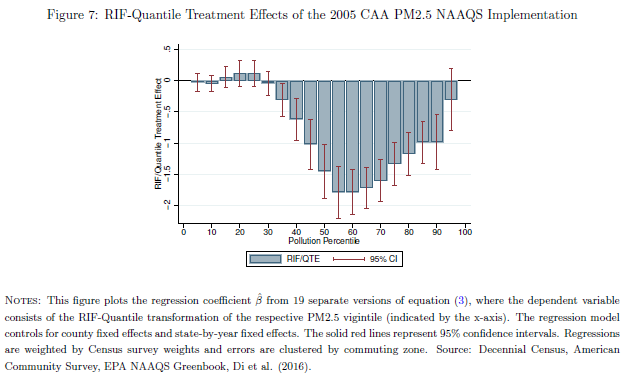
\includegraphics[scale = .7]{F7.png}
  \end{figure}
\end{frame}

\begin{frame}{}
  \begin{figure}
    \centering
    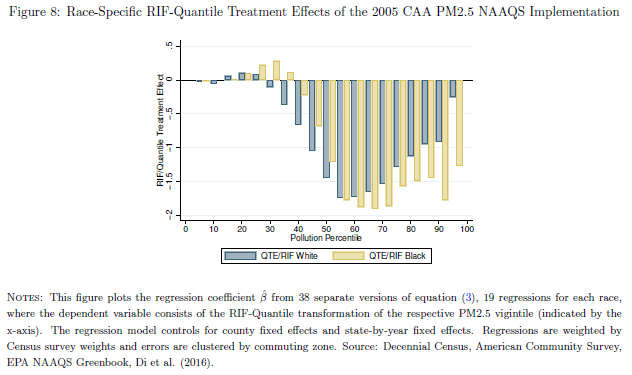
\includegraphics[scale = .65]{F8.png}
  \end{figure}
\end{frame}

\begin{frame}{CAA-Effects on Different Quantiles}
  \begin{itemize}
    \item the most significant effects of the new standards were to improve air quality in areas between the 50th and 90th percentiles of PM2.5 distribution.
    \item On the other hand, the effect size is smaller in the 90th percentile than in the 50-80th percentiles.
    \begin{itemize}
      \item Most severely polluted areas: the San Joaquin Valley or parts of Southern California
    \end{itemize}
    \item Race-specific estimation
    \begin{itemize}
      \item African Americans have seen larger improvements in air quality relative to their non-Hispanic White counterparts (statistically insignificant).
    \end{itemize}
  \end{itemize}
\end{frame}

\begin{frame}{CAA Regulation and Racial Convergence}
  \begin{itemize}
    \item Tract-level population shares by race from the public-use American Community Survey 5-year files enable us to calculate counterfactual changes in pollution exposure.
    \begin{itemize}
      \item The actual gap in 2015 was \SI[per-mode = symbol]{.61}{\micro \gram \per \cubic \meter}
      \item The counterfactual gap is \SI[per-mode = symbol]{.97}{\micro \gram \per \cubic \meter}
      \item The actual change in the Black-White gap between 2005 and 2015 was \SI[per-mode = symbol]{.59}{\micro \gram \per \cubic \meter}
    \end{itemize}
    \item We would have observed a \SI[per-mode = symbol]{.23}{\micro \gram \per \cubic \meter} improvement in the Black-White gap in the absence of the policy
    \item Thus, the CAA can account for over 60\% of the relative improvement in Black-White outcomes.
  \end{itemize}
\end{frame}

\begin{frame}{}
  \begin{figure}
    \centering
    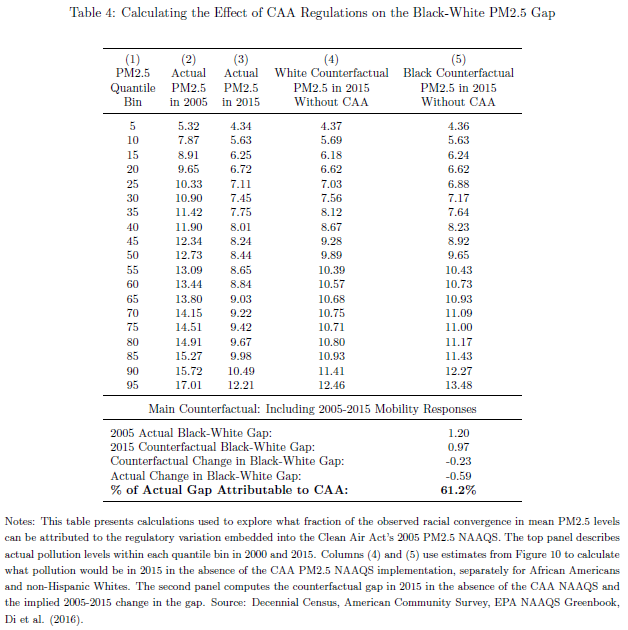
\includegraphics[scale = .5]{T4.png}
  \end{figure}
\end{frame}

\begin{frame}{Mobility Responses}
  \begin{itemize}
    \item Populations shifted in response to the CAA-induced changes in air quality
    \item Non-Hispanic Whites are moving to the set of urban areas
    \begin{itemize}
      \item the areas that saw the largest treatment effects from the Clean Air Act's nonattainment designation are also the areas where the share of African Americans declined the most.
    \end{itemize}
    \item The CAA improved air quality in cities with relatively higher Black population shares, but as those cities became cleaner they also became more White.
  \end{itemize}
\end{frame}

\begin{frame}{}
  \begin{figure}
    \centering
    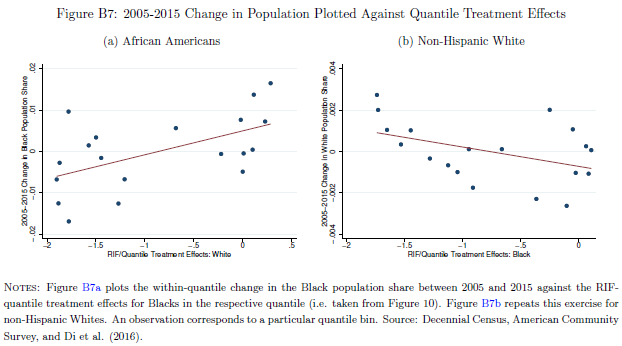
\includegraphics[scale = .6]{FB7.png}
  \end{figure}
\end{frame}

\section{Conclusion}
\frame{\sectionpage}
\begin{frame}{Concluding Remarks}
  \begin{itemize}
    \item This paper add to the small but growing literature using high-resolution, nationwide data on pollution to examine racial differences in potential pollution exposure
    \item Racial gaps in exposure have narrowed at each quantile of the PM2.5 distribution
    \item Fidings suggest that the CAA has likely played a significant role in reducing racial gaps in exposure to air pollution.
  \end{itemize}
\end{frame}

\end{document}
